\msection{\Wasm}
\label{sota:wasm}
%% For the intro
 % In 2014, Alon Zakai and colleagues proposed Emscripten \cite{emscripten}. 
% Emscripten used a strict subset of JavaScript, asm.js, to allow low-level code such as C to be compiled to JavaScript. 
% Asm.js was faster than JavaScript because it limited the language features to those that can be optimized in the LLVM pipeline. 
% Notably, Asm.js demonstrated that client-code could be improved with the right language design and standardization.
% Wasm marked the breaking point of several failed attempts of porting code but JavaScript to the web browser \cite{javaapplet,activex,silverlight}.
% Previous alternatives largely failed to gain traction, primarily due to security concerns and a lack of consensus among browser vendors.
% The announcement of \wasm\ marked the first step into the standardization of bytecode in the web environment. 

% History
The W3C publicly announced the \Wasm(Wasm) language in 2017 as the fourth scripting language supported in all major web browser vendors.
\wasm\ is a binary instruction format for a stack-based virtual machine and was officially consolidated by the work of Haas \etal \cite{Haas_2017} in 2017 and extended by Rossberg \etal in 2018 \cite{10.1145/3282510}. 
It is designed to be fast, portable, self-contained, and secure.

Moreover, WebAssembly has been evolving outside web browsers since its first announcement.
Some works demonstrated that using WebAssembly as an intermediate layer is better in terms of startup time and memory usage than containerization and virtualization \cite{pMendkiServerless, 1244493Jacobsson}. 
Consequently, in 2019, the Bytecode Alliance proposed WebAssembly System Interface (WASI) \cite{WASI}. 
WASI pioneered the execution of \wasm\ with a POSIX system interface protocol, making it possible to execute Wasm closer to the underlying operating system. 
Therefore, it standardizes the adoption of \wasm\ in heterogeneous platforms \cite{bryant2020webassembly}, i.e., IoT and Edge computing \cite{9640153, wen2020wasmachine}.

% Usages of Wasm
%%IMPROVED
Currently, \Wasm serves a variety of functions in browsers, ranging from gaming to cryptomining \cite{Hilbig2021AnES}. 
Other applications include text processing, visualization, media processing, programming language testing, online gambling, bar code and QR code fast reading, hashing, and PDF viewing. 
On the backend, \Wasm notably excels in short-running tasks. 
As such, it is particularly suitable for Function as a Service (FaaS) platforms like Cloudflare and Fastly.
The broad spectrum of applicability and the rapid adoption of \Wasm have resulted in demands for additional features. 
However, not all these demands align with its original specification.
Thus, since the introduction of \Wasm, various extensions have been proposed for standardization. 
For instance, the SIMD proposal enables the execution of vectorized instructions in \Wasm. 
To become a standard, a proposal must fulfill certain criteria, including having a formal specification and at least two independent implementations, e.g., two different engines. 
Notably, even after adoption, new extensions are optional; the core \Wasm remains untouched and continues to be referred to as version 1.0. 
The subsequent text in this chapter focuses specifically on \Wasm version 1.0. 
However, the tools, techniques, and methodologies discussed are applicable to future \Wasm versions.





%\todo{TBD: Some words about the evergreen method and how to extend Wasm?}
%\vspace{-1.5cm}
% How to generate
%\msubsection{\Wasm's generation and binary format}
%\todo{Replace by Rust example}
%\todo{Annotate the Wasm code with the sections offset and length}
%\todo{Instantiate each one of the previously mentioned concepts}
%\todo{Improve some metadata, size of the code, etc}
%\todo{FIX: linerefs}

\msubsection{From source code to \Wasm}

\Wasm programs are compiled from source languages like C/C++, Rust, or Go, which means that it can benefit from the optimizations of the source language compiler.
The resulting \wasm program is like a traditional shared library, containing instruction codes, symbols, and exported functions. 
A host environment is in charge of complementing the Wasm program, such as providing external functions required for execution within the host engine. 
For instance, functions for interacting with an HTML page's DOM are imported into the Wasm binary when invoked from JavaScript code in the browser. 


\begin{minipage}[h]{0.9\textwidth}
    \begin{minipage}[t]{1.0\linewidth}
        \lstset{language=C,caption={Example C program which includes heap allocation, external function usage, and a function definition featuring a loop, conditional branching, function calls, and memory accesses.  },
        label=CExample1,
        breaklines=true, 
        basicstyle=\small\ttfamily,
        captionpos=b,
        frame=b,
        numbers=left,
        postbreak=\mbox{\textcolor{red}{$\hookrightarrow$}\space},
        escapeinside={(*@}{@*)}
        }
    \input{sota/code/code.c}
    \end{minipage}
\end{minipage}


In \autoref{CExample1} and \autoref{WASMExample}, we present a C program alongside its corresponding WebAssembly binary. 
The C function encompasses various elements such as heap allocation, external function usage, and a function definition that includes a loop, conditional branching, function calls, and memory accesses.
The Wasm code shown in \autoref{WASMExample} is displayed in its textual format, known as WAT\footnote{The WAT text format is primarily designed for human readability and for low-level manual editing.}.
The static memory declared in line 2 of \autoref{CExample1} is allocated within the Wasm binary's linear memory, as illustrated in line 47 of \autoref{WASMExample}.
The function prototype in line 5 of \autoref{CExample1} is converted into an imported function, as seen in line 8 of \autoref{WASMExample}.
The main function, spanning lines 7 to 14 in \autoref{CExample1}, is transcribed into a Wasm function covering lines 12 to 38 in \autoref{WASMExample}. Within this function, the translation of various C language constructs into Wasm can be observed.
For instance, the \texttt{for} loop found in line 8 of \autoref{CExample1} is mapped to a block structure in lines 17 to 31 of \autoref{WASMExample}. 
The loop's breaking condition is converted into a conditional branch, as shown in line 25 of \autoref{WASMExample}.


There exist several compilers that turn source code into \Wasm binaries. 
For example, LLVM compiles to \Wasm as a backend option since its 7.1.0 release\toolcite{https://github.com/llvm/llvm-project/releases/tag/llvmorg-7.1.0}, supporting a diverse set of frontend languages like C/C++, Rust, Go, and AssemblyScript\footnote{A subset of the TypeScript language}.
Significantly, a study by Hilbig \cite{Hilbig2021AnES} reveals that 70\% of \Wasm binaries are generated using LLVM-based compilers. 
The main advantage of using LLVM is that it provides a modular and state-of-the-art optimization infrastructure for \Wasm binaries.
In parallel, the KMM framework\toolcite{https://kotlinlang.org/docs/wasm-overview.html} has incorporated \Wasm as a compilation target.



A recent trend in the \Wasm ecosystem involves porting various programming languages by converting both the language's engine or interpreter and the source code into a \Wasm program. 
For example, Javy\toolcite{https://github.com/bytecodealliance/javy} encapsulates JavaScript code within the QuickJS interpreter, demonstrating that direct source code conversion to \Wasm isn't always required. 
If an interpreter for a specific language can be compiled to \Wasm, it allows for the bundling of both the interpreter and the language into a single, isolated \Wasm binary. 
Similarly, Blazor\toolcite{https://dotnet.microsoft.com/en-us/apps/aspnet/web-apps/blazor} facilitates the execution of .NET Common Intermediate Language (CIL) in \Wasm binaries for browser-based applications. 
However, packaging the interpreter and the code in one single standalone \Wasm binary is still immature and faces challenges.
For example, the absence of JIT compilation for the "interpreted" code makes it less suitable for long-running tasks \cite{10.1145/3593434.3593454}. 
On the other hand, it proves effective for short-running tasks, particularly those executed in Edge-Cloud computing platforms.

\begin{minipage}[hbtp]{0.9\textwidth}
  

    \begin{minipage}[t]{1.0\linewidth}
    \lstset{
        language=WAT,
        caption={ Refer to \autoref{CExample1} for the Rust code example. This example showcases the translation from Rust to \wasm. For clarity, we have marked elements and portions of the \Wasm binary as comments.},
        style=WATStyle,
        breaklines=true, 
        %stepnumber=0,
        captionpos=b,
        frame=b,
        escapeinside={(*@}{@*)},
        numbers=none,
        postbreak=\mbox{\textcolor{red}{$\hookrightarrow$}\space},
        label=WASMExample}
    %
    \input{sota/code2/fibo.shortest.wat}
    %\end{lstlisting}
    \end{minipage}
\end{minipage}



\msubsection{\Wasm's binary format}
\label{background:wasm:binary}

The Wasm binary format is close to machine code and already optimized, being a consecutive collection of sections.
In \autoref{background:wasm:fig:section} we show the binary format of a Wasm section.
A Wasm section starts with a 1-byte section ID, followed by a 4-byte section size, and concludes with the section content, which precisely matches the size indicated earlier.
A \wasm binary contains sections of 13 types, each with a specific semantic role and placement within the module. 
For instance, the \emph{Custom Section} stores metadata like the compiler used to generate the binary, while the \emph{Type Section} contains function signatures that serve to validate the \emph{Function Section}. 
The \emph{Import Section} lists elements imported from the host, and the \emph{Function Section} details the functions defined within the binary. 
Other sections like \emph{Table, Memory, and Global Sections} specify the structure for indirect calls, unmanaged linear memories, and global variables, respectively. 
\emph{Export, Start, Element, Code, Data, and Data Count Sections} handle aspects ranging from declaring elements for host engine access to initializing program state, declaring bytecode instructions per function, and initializing linear memory. 
Each of these sections must occur only once in a binary and can be empty.
For clarity, we also annotate sections as comments in the Wasm code in \autoref{WASMExample}.
    

\begin{figure}[h]
    \centering
    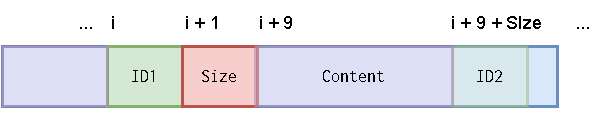
\includegraphics[width=0.5\linewidth]{figures/section.pdf}
    \caption{Memory byte representation of a \Wasm binary section, starting with a 1-byte section ID, followed by an 8-byte section size, and finally the section content.}
    \label{background:wasm:fig:section}
\end{figure}

A \wasm binary can be processed efficiently due to its organization into a contiguous array of sections. 
For instance, this structure permits compilers to expedite the compilation process either through parallel parsing or by disregarding \emph{Custom Sections}. 
Moreover, the \emph{Code Section}'s instructions are further compacted through the use of the LEB128\toolcite{https://en.wikipedia.org/wiki/LEB128} encoding. 
Consequently, Wasm binaries are not only fast to validate and compile, but also swift to transmit over a network.

\msubsection{\Wasm's runtime}
\label{background:wasm:execution}

The \Wasm's runtime characterizes the behavior of \wasm programs during execution. 
This section describes the main components of the \Wasm runtime, namely the execution stack, functions, memory model, and execution process. 
These components are crucial for understanding both the \Wasm's control-flow and the analysis of \Wasm binaries.


\wrule{Execution Stack:} At runtime, \Wasm engines instantiate a \Wasm module. 
This module is a runtime representation of a loaded and initialized \Wasm binary described in \autoref{background:wasm:binary}. 
The primary component of a module instance is its Execution Stack. 
The Execution Stack stores typed values, labels, and control frames. 
Labels manage block instruction starts and loop starts.
Control frames manage function calls and function returns.
Values within the stack can only be static types.
These types include \texttt{i32} for 32-bit signed integers, \texttt{i64} for 64-bit signed integers, \texttt{f32} for 32-bit floats, and \texttt{f64} for 64-bit floats. 
Abstract types such as classes, objects, and arrays are not supported natively. 
Instead, these types are abstracted into primitive types during compilation and stored in linear memory.


\wrule{Functions:} At runtime, \Wasm functions are closures over the module instance, grouping locals and function bodies.
Locals are typed variables that are local to a specific function invocation.
A function body is a sequence of instructions that are executed when the function is called.
Each instruction either reads from the execution stack, writes to the execution stack, or modifies the control-flow of the function.
Recalling the example \wasm binary previously showed, the local variable declarations and typed instructions that are evaluated using the stack can be appreciated between Line 12 and Line 38 in \autoref{WASMExample}. 
Each instruction reads its operands from the stack and pushes back the result. 
Notice that, numeric instructions are annotated with its corresponding type.
In the case of \autoref{WASMExample}, the result value of the main function is the calculation of the last instruction, \texttt{i32.add} in line 38. 
As the listing also shows, instructions are annotated with a numeric type.


\wrule{Memory model:} A WebAssembly module instance incorporates three key types of memory-related components: linear memory, local variables and global variables. 
These components can either be managed solely by the host engine or shared with the \Wasm binary itself. 
This division of responsibility is often categorized as \emph{managed} and \emph{unmanaged} memory \cite{usenixWasm2020}. 
Managed refers to components that are exclusively modified by the host engine at the lowest level, e.g. when the \Wasm binary is JITed, while unmanaged components can also be altered through  \Wasm opcodes.
First, modules may include multiple linear memory instances, which are contiguous arrays of bytes. 
These are accessed using 32-bit integers (\texttt{i32}) and are shareable only between the initiating engine and the \Wasm binary. 
Generally, these linear memories are considered to be unmanaged, e.g., line 21 of \autoref{WASMExample} shows an explicit memory access opcode. 
Second, there are global instances, which are variables accompanied by values and mutability flags (see example in line 42 of \autoref{WASMExample}). 
These globals are managed by the host engine, which controls their allocation and memory placement completely oblivious to the \Wasm binary scope. 
They can only be accessed via their declaration index, prohibiting dynamic addressing. 
Third, local variables are mutable and specific to a given function instance. 
They are accessible only through their index relative to the executing function and are part of the data managed by the host engine.


\wrule{\Wasm module execution:}
While a \Wasm binary could be interpreted, the most practical approach is to JIT compile it into machine code.
The main reason is that \Wasm is optimized and closely aligned with machine code, leading to swift JIT compilation for execution.
Browser engines such as V8\toolcite{https://chromium.googlesource.com/v8/v8.git} and SpiderMonkey\toolcite{https://spidermonkey.dev/} utilize this strategy when executing \Wasm binaries in browser clients.
Once JITed, the \Wasm binary operates within a sandboxed environment, accessing the host environment exclusively through imported functions.
The communication between the host and the \Wasm module execution is typically facilitated by trampolines in the JITed machine code.

\wrule{\Wasm standalone engines:}
While initially intended for browsers, \Wasm has undergone significant evolution, primarily due to WASI\cite{WASI}.
WASI establishes a standardized POSIX-like interface for interactions between \Wasm modules and host environments.
Compilers can generate \wasm binaries that implement WASI, which allows execution in standalone engines.
These binaries can then be executed by standalone engines across a variety of environments, including the cloud, servers, and IoT devices \cite{makitalo2021webassembly}.
Similarly to browsers, these engines often translate \Wasm into machine code via JIT compilation, ensuring a sandboxed execution process.
Standalone engines such as WASM3\toolcite{https://github.com/wasm3/wasm3}, Wasmer\toolcite{https://wasmer.io/}, Wasmtime\toolcite{https://github.com/bytecodealliance/wasmtime}, WAVM\toolcite{https://github.com/WAVM/WAVM}, and Sledge\cite{Sledge} have been developed to support both \Wasm and WASI.
In a related development, Singh et al.\cite{WARDuino2019} have created a \Wasm virtual machine specifically designed for Arduino-based devices.




\msubsection{\Wasm's control-flow}
\label{wasm:control_flow}

A \Wasm function groups instructions into blocks, with the function's entrypoint acting as the root block. 
In contrast to conventional assembly code, control-flow structures in Wasm leap between block boundaries rather than arbitrary positions within the code, effectively prohibiting \texttt{goto}s to random code positions. 
Each block may specify the needed execution stack state before execution as well as the resultant execution stack state once its instructions have been executed.
Typically, the execution stack state is simply the quantity and numeric type of values on the stack. 
This stack state is used to validate the binary during compilation and to ensure that the stack is in a valid state before the execution of the block's instructions.
Blocks in Wasm are explicit (see instructions \texttt{block} and \texttt{end} in lines 16 and 34 of \autoref{WASMExample}), delineating where they commence and conclude.
By design, a block cannot reference or execute code from external blocks.


During runtime, \Wasm break instructions can only jump to one of its enclosing blocks. 
Breaks, except for those within loop constructions, jump to the block's end and continue to the next immediate instruction. 
For instance, after line 34 of \autoref{WASMExample}, the execution would proceed to line 35. 
Within a loop, the end of a block results in a jump to the block's beginning, thus restarting the loop. 
For example, if line 30 of \autoref{WASMExample} evaluates as false, the next instruction to be executed in the loop would be line 18. 
\autoref{background:wasm:block} provides an example for better understanding, comparing a standard block and a loop block in a Wasm function.


\begin{minipage}{0.95\linewidth}
   
   \begin{minipage}{0.45\linewidth}
      \lstset{
      language=WAT,
      style=WATStyle,
      breaklines=true, 
      %stepnumber=0,
      escapeinside={(*@}{@*)},
      numbers=none,
      postbreak=\mbox{\space},
      label=BlockExample}

   \begin{lstlisting}    
block
   block
      br 1 (*@\tikzmarkMap{2}{}{8.5}{2}{2cm}@*) ; Jump instructions are annotated with the depth of the block they jump to; 
   end (*@\tikzmarkMap{7}{}{8.5}{0}{2cm}@*)
end (*@\tikzmarkMap{1}{}{8}{3}{2cm}@*)
... (*@\tikzmarkMap{9}{}{8.5}{2}{2cm}@*)
   \end{lstlisting}
   \end{minipage}\hspace{1mm}
   \begin{minipage}{0.44\linewidth}
   \lstset{
      language=WAT,
      style=WATStyle,
      breaklines=true, 
      %stepnumber=0,
      escapeinside={(*@}{@*)},
      numbers=none,
      postbreak=\mbox{\space},
      label=LoopExample}

   \begin{lstlisting}    
loop (*@\tikzmarkMap{6}{}{8.5}{2}{2cm}@*)
   ...
   br 0 (*@\tikzmarkMap{5}{}{8.5}{2}{2cm}@*) ;first-order break;
   ... 
end (*@\tikzmarkMap{3}{}{8.5}{2}{2cm}@*) ; end instructions break the block and jump to next instruction; 
... (*@\tikzmarkMap{4}{}{8.5}{-2}{2cm}@*)
   \end{lstlisting}
   \end{minipage}
   \begin{tikzpicture}[remember picture,overlay]

      %\path (2.west) edge[<-, black] (1.west);
      %\path (3.west) edge[<-,  black] (4.west);
   
      \path (1.west) edge[<-, bend right, black] (2.west);
      %\path (1.west) edge[<-, bend right, gray] (7.west);
      %\path (9.west) edge[<-, bend right, gray] (1.west);
   
      \path (4.west) edge[<-, bend right, gray] (3.west);
      \path (6.west) edge[<-, bend left, black] (5.west);
      %\path (9.east) edge[<-, bend right, black] (4.east);
      %\path (7.east) edge[<-, bend right, black] (8.east);
   
      \end{tikzpicture}
      \centering
      \hrule
      \vspace{2mm}
      \captionof{lstlisting}{Example of breaking a block and a loop in \Wasm.}
      \label{background:wasm:block}
\end{minipage}
% Example


Each break instruction includes the depth of the enclosing block as an operand. 
This depth is used to identify the target block for the break instruction. 
For example, in the left-most part of the previously discussed listing, a break instruction with a depth of 1 would jump past two enclosing blocks.
This design hardens the rewriting of \wasm binaries.
For instance, if an outer block is removed, the depth of the break instructions within nested blocks must be updated to reflect the new enclosing block depth.
This is a significant challenge for rewriting tools, as it requires the analysis of the control-flow graph to determine the enclosing block depth for each break instruction.

\msubsection{Security and Reliability for WebAssembly}
\label{background:wasm:analysis}

The WebAssembly ecosystem's expansion needs robust tools to ensure its security and reliability. 
Numerous tools, employing various strategies to detect vulnerabilities in \Wasm programs, have been created to meet this need. 
This paper presents a review of the most relevant tools in this field, focusing on those capable of providing security guarantees for \Wasm binaries.

%%ORIGINAL
\wrule{Static analysis:} SecWasm\cite{secwasm} uses information control-flow strategies to identify vulnerabilities in \Wasm binaries. 
Conversely, Wasmati\cite{wasmati} employs code property graphs for this purpose. 
Wasp\cite{Wasp} leverages concolic execution to identify potential vulnerabilities in \Wasm binaries. 
VeriWasm\cite{veriwasm}, an offline verifier designed specifically for native x86-64 binaries JITed from \Wasm, adopts a unique approach. 
While these tools emphasize specific strategies, others adopt a more holistic approach. 
CT-Wasm\cite{ctwasm}, verifies the implementation of cryptographic algorithms in \Wasm. 
Similarly, Vivienne applies relational Symbolic Execution (SE) to \Wasm binaries in order to reveal vulnerabilities in cryptographic implementations\cite{Vivienne}. 
For example, both Wassail\cite{wassail} and WasmA\cite{WasmA} provide a comprehensive static analysis framework for \Wasm binaries. 
However, static analysis tools may have limitations. 
For instance, a newly, semantically equivalent \Wasm binary may be generated from the same source code bypassing or breaking the static analysis \cite{breaking example}.
If the \Wasm input differs from the input used during sound analysis \cite{sound_analysis}, the vulnerability may go unnoticed. 
Thus, there may be a lack of subjects to evaluate the effectiveness of these tools.

\wrule{Dynamic analysis:} Dynamic analysis involves tools such as TaintAssembly\cite{taintassembly}, which conducts taint analysis on \Wasm binaries. 
Fuzzm\cite{fuzzm} identifies vulnerabilities in host engines by conducting property fuzzing through \Wasm binary execution. 
Furthermore, Stiévenart and colleagues have developed a dynamic approach to slicing \Wasm programs based on Observational-Based Slicing (ORBS)\cite{slicing, slicing2}.
This technique aids in debugging, understanding programs, and conducting security analysis.
However, Wasabi\cite{wasabi} remains the only general-purpose dynamic analysis tool for \Wasm binaries, primarily used for profiling, instrumenting, and debugging \Wasm code. 
Similar to static analysis, these tools typically analyze software behavior during execution, making them inherently reactive. 
In other words, they can only identify vulnerabilities or performance issues while pseudo-executing input \wasm programs.
Thus, facing an important limitation on overhead for real-world scenarios. 

%%ORIGINAL
\wrule{Protecting \Wasm binaries and runtimes:}
The techniques discussed previously are primarily focused on reactive analysis of \Wasm binaries.
However, there exist approaches to harden \Wasm binaries, enhancing their secure execution, and fortifying the security of the entire execution runtimes ecosystem. 
For instance, Swivel\cite{Swivel} proposes a compiler-based strategy designed to eliminate speculative attacks on \Wasm binaries, particularly in Function-as-a-Service (FaaS) platforms such as Fastly. 
Conversely, WaVe\cite{wave} introduces a mechanized engine for \Wasm that facilitates differential testing. 
This engine can be employed to detect anomalies in engines running Wasm-WASI programs. 
Much like static and dynamic analysis tools, these tools may suffer from a lack of \Wasm inputs, which could affect the measurement of their effectiveness.


\todo{Isolation without taxation}\url{https://arxiv.org/abs/2105.00033}


%%ORIGINAL
\wrule{\Wasm malware:} Since the introduction of \wasm, the Web has consistently experienced an increase in cryptomalware. 
This rise primarily stems from the shift of mining algorithms from CPUs to \wasm, a transition driven by notable performance benefits \cite{musch2019new}.
Tools such as MineSweeper\cite{Minesweeper}, MinerRay\cite{MinerRay}, and MINOS\cite{MINOS} employ static analysis with machine learning techniques to detect browser-based cryptomalwares.
Conversely, SEISMIC\cite{SEISMIC}, RAPID\cite{RAPID}, and OUTGuard\cite{outguard} leverage dynamic analysis techniques to achieve a similar objective.
VirusTotal\toolcite{https://www.virustotal.com}, a tool incorporating over 60 commercial antivirus systems as black-boxes, is capable of detecting cryptomalware in \wasm binaries.
However, obfuscation studies have exposed their shortcomings, revealing an almost unexplored area for \Wasm that threatens malware detection accuracy.
In concrete, Bahnsali \etal seminal work\cite{10.1145/3507657.3528560} demonstrate that cryptomining algorithm's source code can evade previous techniques through the use of obfuscation techniques.


\msubsection{Open challenges}
\label{background:wasm:challenges} 
Despite progress in \Wasm analysis, numerous challenges remain. 
\Wasm, though deterministic and well-typed by design, boasts an emerging ecosystem susceptible to a variety of security threats. 
First, most existing \Wasm research is reactive, focusing on detecting and fixing vulnerabilities already reported. 
This approach leaves \Wasm binaries and runtime implementations potentially open to unidentified attacks. 
Second, side-channel attacks present a significant risk. 
Genkin et al., for example, illustrated how \Wasm could be manipulated to extract data via cache timing-side channels \cite{Genkin2018DrivebyKC}. 
Furthermore, research conducted by Maisuradze and Rossow demonstrated the potential for speculative execution attacks on \Wasm binaries \cite{ret2spec}. 
Rokicki et al. disclosed the possibility for port contention side-channel attacks on \Wasm binaries in browsers \cite{10.1145/3488932.3517411}. 
Finally, the binaries themselves may be inherently vulnerable. 
For example, studies by Lehmann et al. and Stiévenart et al. suggested that flaws in C/C++ source code could infiltrate \Wasm binaries \cite{usenixWasm2020, DeRoover2022}.
 


This dissertation presents toolsets, approaches and methodologies designed to enhance \Wasm security proactively through Software Diversification.
First, Software Diversification could expand the capabilities of the mentioned tools by incorporating diversified program variants, making it more challenging for attackers to exploit any missed vulnerabilities.
Generated as proactive security, these diversified variants can simulate a broader set of real-world conditions, thereby making \Wasm analysis tools more accurate. 
Second, we noted that current solutions to mitigate side-channel attacks on \Wasm binaries are either specific to certain attacks or need the modification of runtimes, e.g., Swivel as a cloud-deployed compiler.
Software Diversification could mitigate yet-unknown vulnerabilities on \Wasm binaries by generating diversified variants in a platform-agnostic manner.

